\subsection{Solstrålning genom fönster}

Exempel på resultat från beräkningar på solstrålning genom fönster. Beräknat via trial.m i code-mappen.

I figur \ref{fig:sun0101and0601} ses de relevanta vinklar som bildas av solens position den första april, 2012. Den blå linjen i figuren representerar solens vinkel relativt ett fönsters normal (då denna pekar i horisontell sydlig riktning) och kan användas för att uppskatta effekten som solinstrålning bidrar till. Om solens intensitet antas vara konstant $\unit{200}{W/m^2}$ beräknas denna effekt motsvara vad som visas i figur \ref{fig:effekt0101and0601}. Här antas fönstrets area uppgå till $\unit{1.5}{m^2}$, g-värdet för normal solstrålning är ? och värdet p i koden sätts till ?, ty fönstren i den avsedda byggnaden är av typ treglas utan ytbeläggningar.

\begin{figure}[hpbt]
\centering
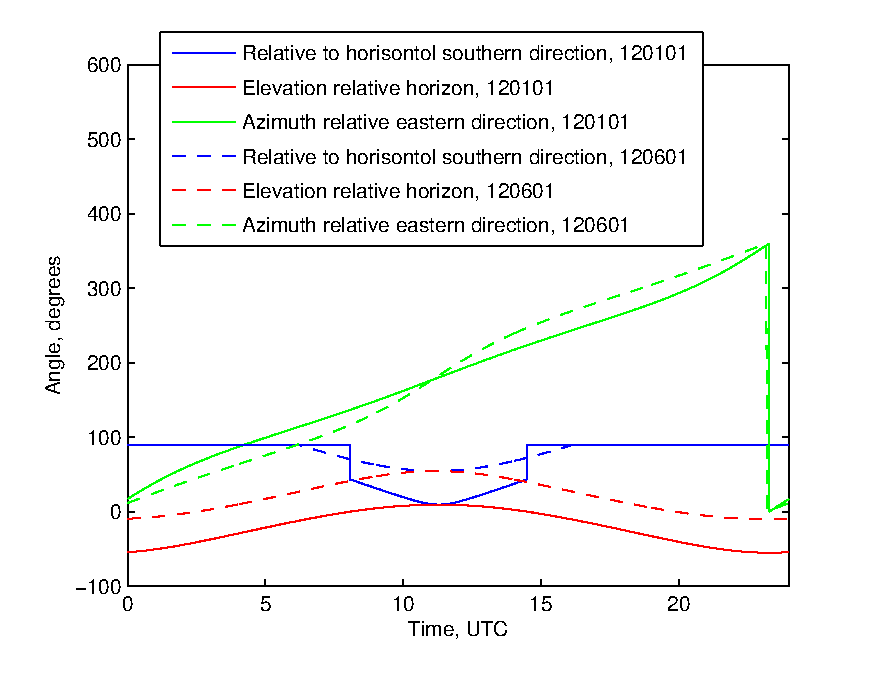
\includegraphics[scale=1]{images/sun0101and0601.eps}
\caption{\label{fig:sun0101and0601} Beräknade vinklar vid Walleriusgatan den första januari 2012 samt den första juni samma år, tid i UTC}
\end{figure}

\begin{figure}[hpbt]
\centering
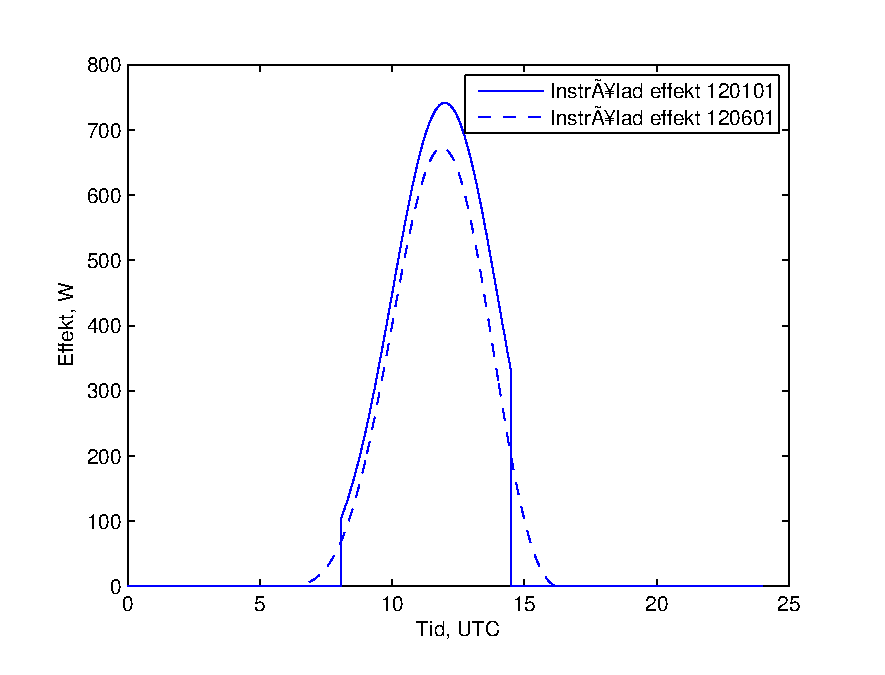
\includegraphics[scale=1]{images/effekt0101and0601.eps}
\caption{\label{fig:effekt0101and0601} Beräknad effekt genom ett fönster vars normal pekar i horisontella sydriktningen, den första januari 2012 samt den första juni samma år. Solens intensitet varierar under dagen enligt den blå kurvan.}
\end{figure}
